\section{Simulations and Results}\label{sec:Results}
All analog simulations were performed in the language of \textit{AIMSpice} in the \textit{AIM-Spice} computer program. All analog simulations were performed in the language \textit{Verilog}, with the editor \textit{VSCode}, compiler \textit{Icarus Verilog} and waveform plotter \textit{gtkwave}.

\subsection{Analog bitcell}
The analog behavior of the bitcell was simulated to show the functionality at different temperatures and with different configurations of slow/fast nmos/pmos transistors, as well as the read-time, the write-time and the leakage current for the SS, TT and FF (TODO: write in theory) configurations. 

\subsubsection{Leakage}
The leakage currents at different configurations:
\begin{figure}
    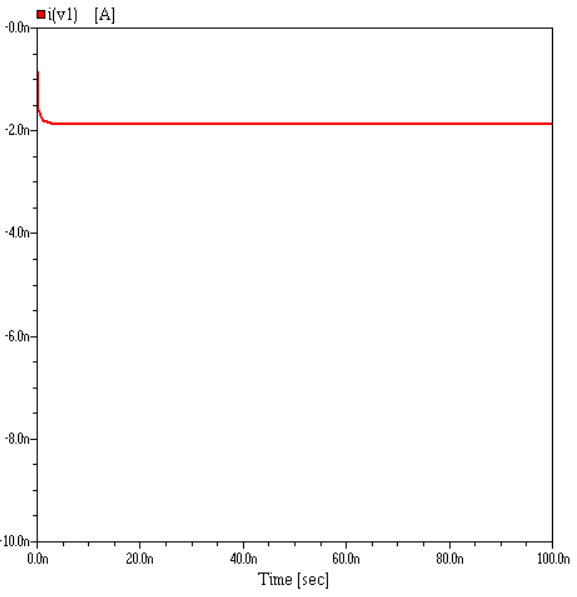
\includegraphics[width=0.3\linewidth]{aimSpice/plots/plotsSS/leak.png}
    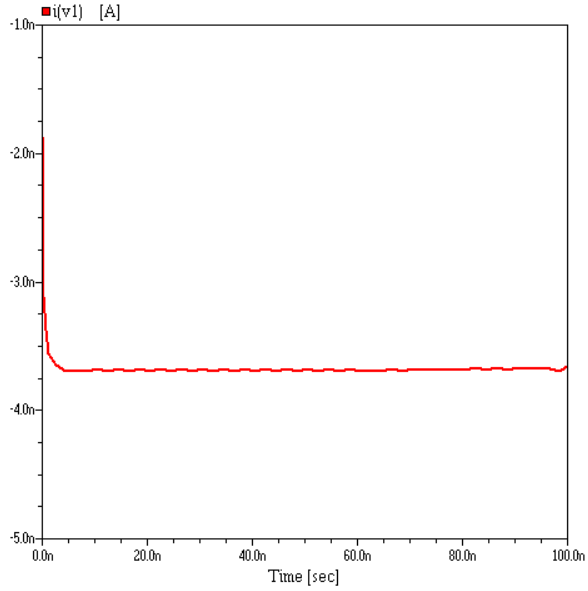
\includegraphics[width=0.3\linewidth]{aimSpice/plots/plotsTT/leak.png}
    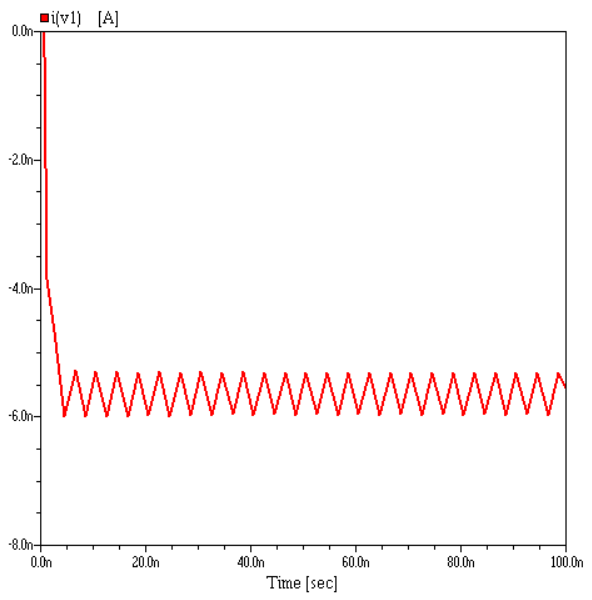
\includegraphics[width=0.3\linewidth]{aimSpice/plots/plotsFF/leak.png}
    \caption{Leakage currents at SS, TT and FF (from left to right)}
    \label{fig:04:leakage}
\end{figure}

\subsection{Digital bitcell}
The bitcell's behaviour was digitally simulated with inputs and outputs as can be observed in \autoref{fig:04:bitcell_tb}.

\begin{figure}
    \centering
    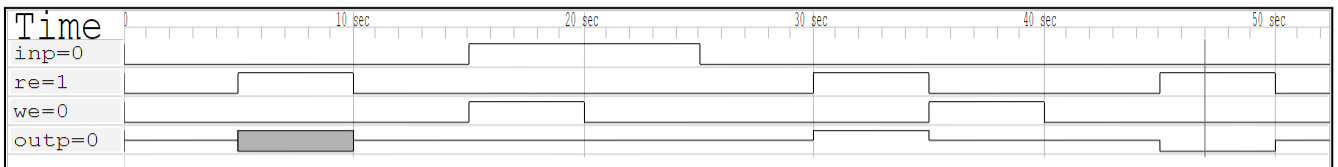
\includegraphics[width=0.9\linewidth]{LaTeX_2/Figures/bitcell_tb.png}
    \caption{Testbench of the bitcell}
    \label{fig:04:bitcell_tb}
\end{figure}

In the testbench we first try to read the bitcell before any value has been set, then we write a logic high, read it, write a logic low, and read that too. 

REN is not shown in the figure, since it is trivial.

\subsection{RAM}



\subsection{FSM}



\subsection{Complete memory module}


